\documentclass{article}
\usepackage[left=2cm,right=2cm,top=2cm,bottom=2cm]{geometry} 
\usepackage{blindtext}
\usepackage{graphicx} 
\usepackage[section]{placeins} 
\usepackage[spanish]{babel}
\usepackage{listings} 
\usepackage{xcolor} 
\usepackage{pdfpages}
\setcounter{secnumdepth}{2}
\usepackage{apacite}

\newcommand*\rbreak{\par\noindent\linebreak}
\graphicspath{{/home/renato/screenshots/math/t3/}}

\begin{document}
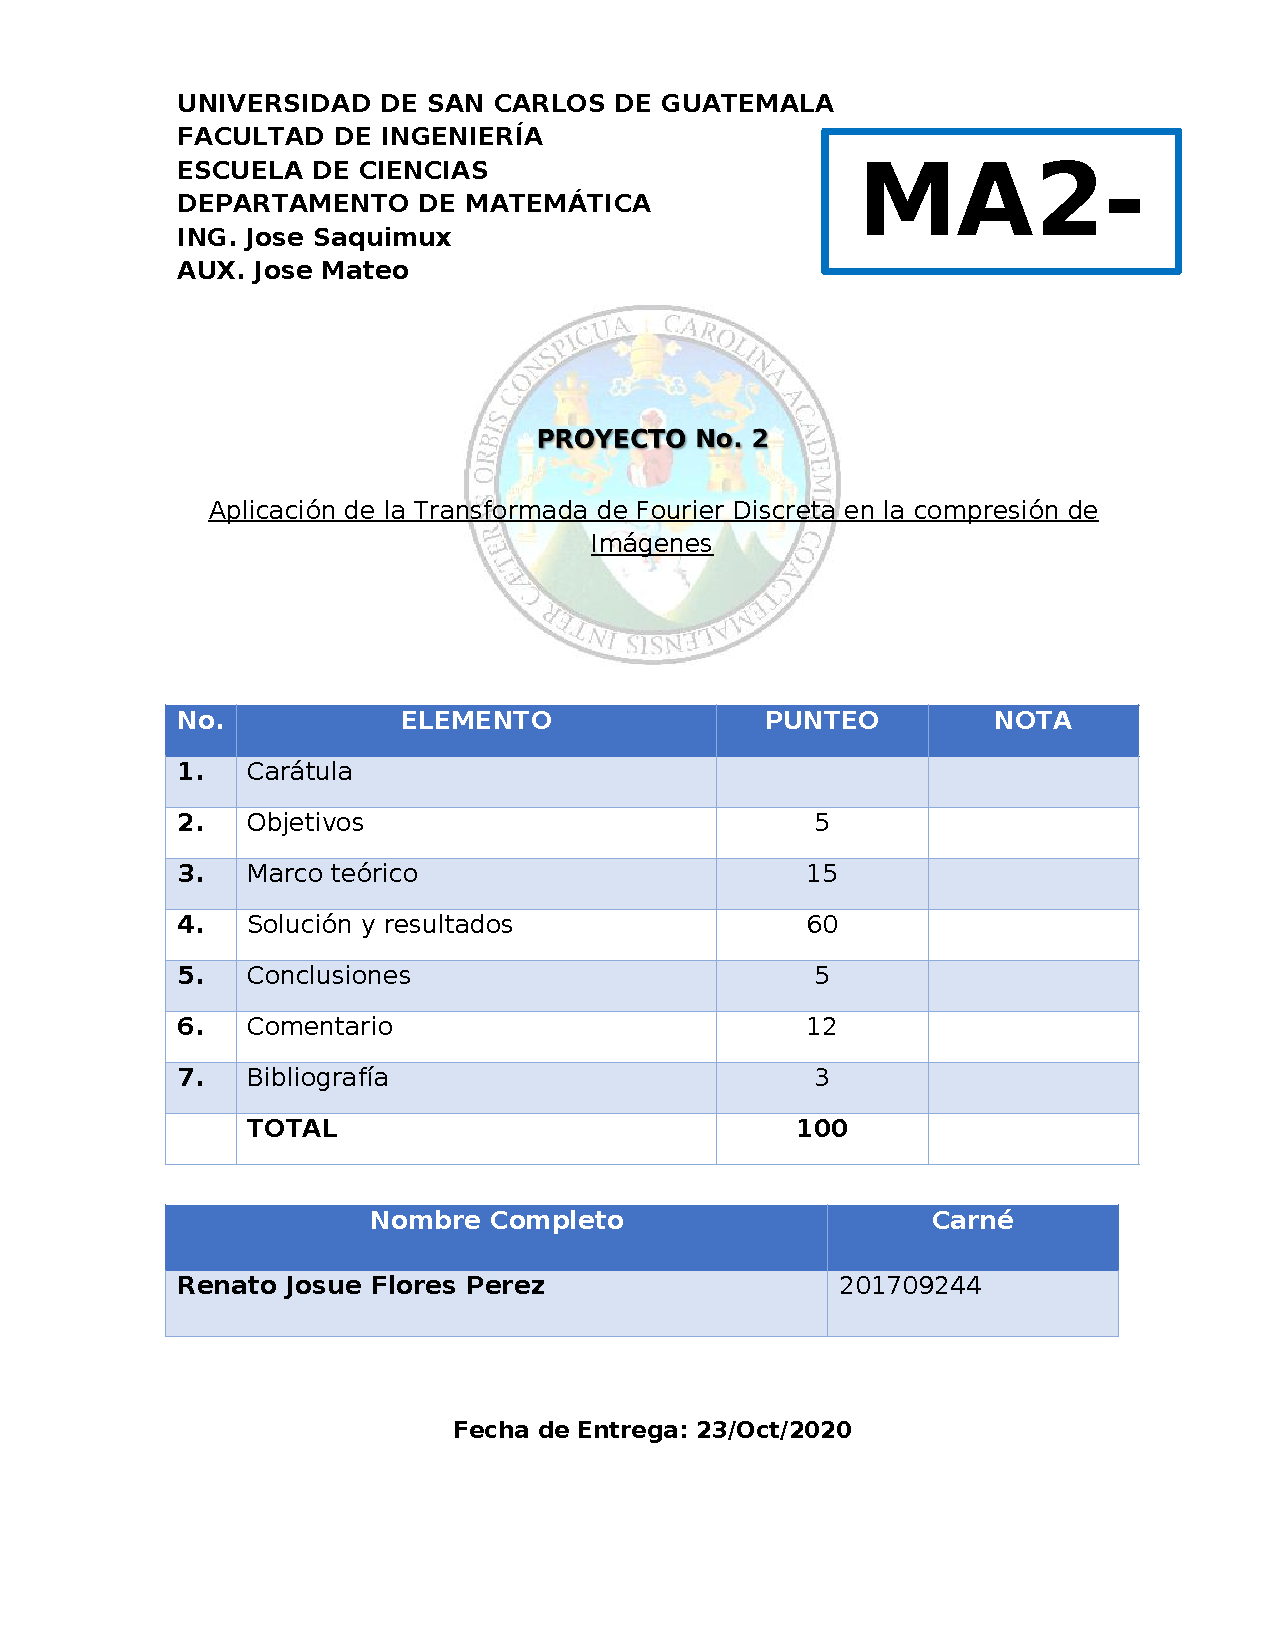
\includepdf{/home/renato/math/projMA2.pdf}	
\section{Marco Teórico}
	En la ingeniería en sistemas es un tanto improbable encontrar
	y analizar señales, por lo que a simple vista parecería que 
	la Transformada de Fourier no tiene aplicación real en este
	campo más que para efectos didácticos o de academia. Sin 
	embargo, cuando se estudia la Transformada Discreta de Fourier
	aparecen muchas aplicaciones, una de las más comúnes 
	es la aplicación de la Transformada Discreta de Fourier (d.c.t)
	por sus siglas en inglés en la compresión de imágenes.\\\\
	Esto se logra expresando la imágen como una matriz de 
	pixeles donde cada pixel tiene asociado un nivel de brillo.
	Mientras con todo el brillo, el pixel se visualiza blanco y 
	con 0 brillo, el pixel se visualiza negro.\\
	En este documento únicamente se trabajan imágenes en esta
	escala simple (blanco y negro) aún si en teoría sería posible
	generalizar este procedimiento para escalas de color 
	más complejas que involucran a todos los colores. \\\\
	
	Para comenzar, debemos definir la d.c.t: \\
	La d.c.t de una sequencia definida $ f[n], n = 0,1,2...N-1;$
	es otra secuencia  $F[k]$ que también tiene N términos 
	definida como: \\\\
	$ F[k] = N^{0.5} \sum_{n=0}^{N - 1} f[n] \cos{\left(\frac{\pi k \left(n + 0.5\right)}{N} \right)}; para k = 0,1,2,3..., N-1 $\\
	Ahora bien, la definición de la transformada como tal no es
	de mucha utilidad al aplicarla con el manejo de imágenes, ya 
	que estas son bi-dimensionales. Sin embargo, es 
	posible extender la definición de la d.c.t para 2 dimensiones
	obteniendo:\\\\
	$F[k,l] = 
\sqrt{M N} \sum_{n=0}^{N - 1} \cos{\left(\frac{\pi k \left(n + 0.5\right)}{N} \right)} \sum_{m=0}^{M - 1} f[n,m] \cos{\left(\frac{\pi l \left(m + 0.5\right)}{M} \right)}	
	$\\

	Empleando esta definición, es posible aplicarla a una 
	imágen donde la primera dimensión (k)
	es la posición en x de un pixel p,
	y la segunda dimensión (l) la posición en y.
\section{Objetivos}
	\begin{itemize}
		\item Comprimir una imágen de tamaño
			arbitriario para ahorrar espacio 
			de almacenamiento.
		\item Perder la menor cantidad posible de calidad
			de imagen en el proceso.
	\end{itemize}
\section{Resolución}
Como se expuso anteriormente, es posible interpretar una imágen
como una matriz donde, el valor de cada punto en la matriz 
es la cantidad de brillo asociada a un pixel de la imágen.
Es posible entonces aplicar la d.c.t. a dicha matriz
para de esta forma contrastar re-ordenar los pixeles de modo
que se puedan agrupar aquellos pixeles con grandes concentraciones.
De este modo, es posible reducir el tamaño de la imágen al recotar
una parte de la matriz transformada, que tanto se corta esta matriz
afectara que tanta calidad de la imágen se perderá. Sin embargo
la pérdida de calidad en la imágen es inevitable para su compresión, 
esta se ve re-compensada por su disminución en tamaño. Dependiendo 
de la importancia de la imágen y la cantidad disponible de 
almacenamiento, se decide cuanto truncar de la matriz resultante. \\
Una vez se desee observar la imágen original, basta
con aplicar la d.c.t inversa a la matriz almacenada, reordenando 
cada pixel nuevamente en su posición original, sin embargo algunos
pixeles no se van a encontrar puesto que se desecharon en el paso 
anterior. Esta falta de pixeles hace que la imagen se vea un 
poco borrosa.
\section{Conclusiones}
\begin{itemize}
	\item La pérdida de calidad y nitidez de la imágen luego de 
	su compresión es inevitable. Sin embargo, el ahorro en 
	almacenamiento físico es de gran utilidada.
\item La idea que se desea expresar capturada en la imágen no 
	se pierde, aún si esta disminuye en nítidez.
\end{itemize}
	

\section{Comentario}
Si bien este método podrá parecer innovador y una excelente idea, 
últimamente está cayendo en desuso por la mayoría del público general,
pues el costo de almacenamiento digital es extremadamente barato 
en la actualidad. Tan asi, que es mucho mas importante conservar 
e incluso aumentar la nítidez de una imágen que ahorrar tamaño de 
almacenamiento digital. Este método es de hecho muy antiguo, cerca
del año 2005, en aquel entonces, el almacenamiento digital aún era
un recurso relativamente preciado. Sin embargo, con la existencia
actual de Terabytes de almacenamiento por costos relativamente bajos, 
la atención en métodos de compresión se ha desvíado un poco. Y puesto
que este método en particular sacrifica parte de la nítidez de la imágen
en su proceso, será muy díficil justificar su implementación en 
nuevas aplicaciones de hoy día.
%Remember to cite all used books at the end like so:
%~\cite{BobsBook01}
%Aftewards you must re-compile the bibliography like so:
%!bibtex proyecto2
%Then delete the citations and re-compile pdflatex like so:
%!pdflatex -synctex=1 -interaction=nonstopmode %
\bibliographystyle{apacite}
\bibliography{proyecto2.bib}
\end{document}
